\documentclass{article}
\usepackage[utf8x]{inputenc}
\usepackage{ucs}
\usepackage{amsmath} 
\usepackage{amsfonts}
\usepackage{upgreek}
\usepackage[english,russian]{babel}
\usepackage{graphicx}
\usepackage{float}
\usepackage{textcomp}
\usepackage{hyperref}
\usepackage{geometry}
  \geometry{left=2cm}
  \geometry{right=1.5cm}
  \geometry{top=1cm}
  \geometry{bottom=2cm}
\usepackage{tikz}
\usepackage{ccaption}
\usepackage{multicol}

\usepackage{listings}
%\setlength{\columnsep}{1.5cm}
%\setlength{\columnseprule}{0.2pt}


\begin{document}
\pagenumbering{gobble}

\lstset{
  language=C,                % choose the language of the code
  basicstyle=\linespread{1.1}\ttfamily,
  columns=fixed,
  fontadjust=true,
  basewidth=0.5em,
  keywordstyle=\color{blue}\bfseries,
  commentstyle=\color{gray},
  stringstyle=\ttfamily\color{orange!50!black},
  showstringspaces=false,
  %numbers=false,                   % where to put the line-numbers
  numbersep=5pt,
  numberstyle=\tiny\color{black},
  numberfirstline=true,
  stepnumber=1,                   % the step between two line-numbers.        
  numbersep=10pt,                  % how far the line-numbers are from the code
  backgroundcolor=\color{white},  % choose the background color. You must add \usepackage{color}
  showstringspaces=false,         % underline spaces within strings
  captionpos=b,                   % sets the caption-position to bottom
  breaklines=true,                % sets automatic line breaking
  breakatwhitespace=true,         % sets if automatic breaks should only happen at whitespace
  xleftmargin=.2in,
  extendedchars=\true,
  keepspaces = true,
  frame=tlbr,
  framesep=8pt,
  framerule=0pt,
}
\lstset{literate=%
   *{0}{{{\color{red!20!violet}0}}}1
    {1}{{{\color{red!20!violet}1}}}1
    {2}{{{\color{red!20!violet}2}}}1
    {3}{{{\color{red!20!violet}3}}}1
    {4}{{{\color{red!20!violet}4}}}1
    {5}{{{\color{red!20!violet}5}}}1
    {6}{{{\color{red!20!violet}6}}}1
    {7}{{{\color{red!20!violet}7}}}1
    {8}{{{\color{red!20!violet}8}}}1
    {9}{{{\color{red!20!violet}9}}}1
}

\definecolor{solcolor}{RGB}{226,240,245}

\title{Семинар \#4: Функции. Решения. \vspace{-5ex}}\date{}\maketitle
\section*{Часть 1: Функции без возвращаемого значения}
Функция \texttt{max} из примера ниже вычисляет максимум 2-х чисел и возвращает его.\\

Помимо функций с возвращаемым значением можно написать и функцию, которая ничего не возвращает. Например, \texttt{print\_n\_times} -- печатает число \texttt{n} раз и ничего не возвращает. У функций, которые ничего не возвращают на месте возвращаемого типа стоит ключевое слово \texttt{void}. Такие функции не требуют оператора \texttt{return}, однако его всё равно можно использовать для выхода из функции.
\begin{lstlisting}
#include <stdio.h>
int max(int a, int b) {
    if (a > b)
        return a;
    return b;
}

void print_n_times(int a, int n) {
    for (int i = 0; i < n; ++i) {
        printf("%i ", a);
    }
}

int main() {
    printf("%i\n", max(5, 7));
    print_n_times(7, 3);
}
\end{lstlisting}

\subsubsection*{Задачи:}
\begin{enumerate}
\item Вызовите функцию \texttt{print\_n\_times} из функции \texttt{main}, чтобы 10 раз напечатать на экран число \texttt{123}.
\item Напишите функцию \texttt{void print\_even\_numbers(int a, int b)}, которая будет печатать все четные числа от \texttt{a} до \texttt{b}. Вызовите эту функцию из функции \texttt{main}.

\item Напишите функцию \texttt{void print\_rectangle(int a, int b)}, которая будет печатать прямоугольник из звёздочек \texttt{*}.  Например, если эта функция будет вызвана с аргументами \texttt{4} и \texttt{3}, то функция должна напечатать:
\begin{verbatim}
****
****
****
\end{verbatim}
Вызовите эту функцию из функции \texttt{main} с различными аргументами.
\item Напишите функцию \texttt{void multi(int type, int a, int b)}, которая, в зависимости от переменной \texttt{type}, должна делать различные вещи. При \texttt{type == 1}, она должна вызывать функцию  \texttt{print\_even\_numbers}. При \texttt{type == 2}, она должна вызывать функцию  \texttt{print\_n\_times}. При \texttt{type == 3}, она должна вызывать функцию  \texttt{print\_rectangle}. При ином другом значении \texttt{type}, она должна просто печатать \texttt{Error!}. Протестируйте вашу функцию.
\end{enumerate}
\begin{lstlisting}[backgroundcolor = \color{solcolor}]
#include <stdio.h>
void print_n_times(int a, int n) {
    for (int i = 0; i < n; ++i) {
        printf("%i ", a);
    }
    printf("\n");
}

void print_even_numbers(int a, int b) {
    if (a % 2)
        a++;
    for (int i = a; i <= b; i += 2)
        printf("%i ", i);
    printf("\n");
}
void print_rectangle(int a, int b) {
    for (int i = 0; i < a; ++i) {
        for (int j = 0; j < b; ++j)
            printf("*");
        printf("\n");
    }
}

void multi(int type, int a, int b) {
    if (type == 1)
        print_even_numbers(a, b);
    else if (type == 2)
        print_n_times(a, b);
    else if (type == 3)
        print_rectangle(a, b);
    else
        printf("Error!\n");
}

int main() {
    multi(1, 2, 8);
    multi(2, 2, 8);
    multi(3, 2, 8);
}
\end{lstlisting}
\newpage
\section*{Часть 2: Рекурсия}
Рекурсивная функция -- это функция, которая вызывает саму себя.  В примере ниже функция \texttt{counter} -- рекурсивная. Если этой функции передать, скажем, число \texttt{5}, то она напечатает это число и вызовет функцию \texttt{counter}, передав ей число \texttt{4}. Так будет продолжаться пока число не дойдёт до \texttt{0}.
\begin{lstlisting}
#include <stdio.h>
void counter(int n) {
    if (n <= 0) {
        return;
    }
    printf("%i ", n);
    counter(n - 1);
}
int main() {
    counter(10);
}
\end{lstlisting}

\subsubsection*{Задачи:}
\begin{itemize}
\item Немного измените функцию \texttt{counter} чтобы она печатала числа с шагом 2.

\begin{lstlisting}[backgroundcolor = \color{solcolor}]
void counter(int n) {
    if (n <= 0) {
        return;
    }
    printf("%i ", n);
    counter(n - 2);
}
\end{lstlisting}

\item Немного измените функцию \texttt{counter} чтобы она делила число \texttt{n} нацело на 2 при каждом рекурсивном вызове.

\begin{lstlisting}[backgroundcolor = \color{solcolor}]
void counter(int n) {
    if (n <= 0) {
        return;
    }
    printf("%i ", n);
    counter(n / 2);
}
\end{lstlisting}

\item Немного измените изначальную функцию \texttt{counter} чтобы она печатала числа по возрастанию. 
\begin{lstlisting}[backgroundcolor = \color{solcolor}]
void counter(int n) {
    if (n <= 0) {
        return;
    }
    counter(n - 1);
    printf("%i ", n);
}
\end{lstlisting}
Для лучшего понятия, что происходит в этой функциях \texttt{counter} рассмотрим на схемы вызовов рекурсивной функции. Для изначальной функции \texttt{counter} она выглядит следующим образом (предположим, что вызываем \texttt{counter(4)}):


\begin{center}
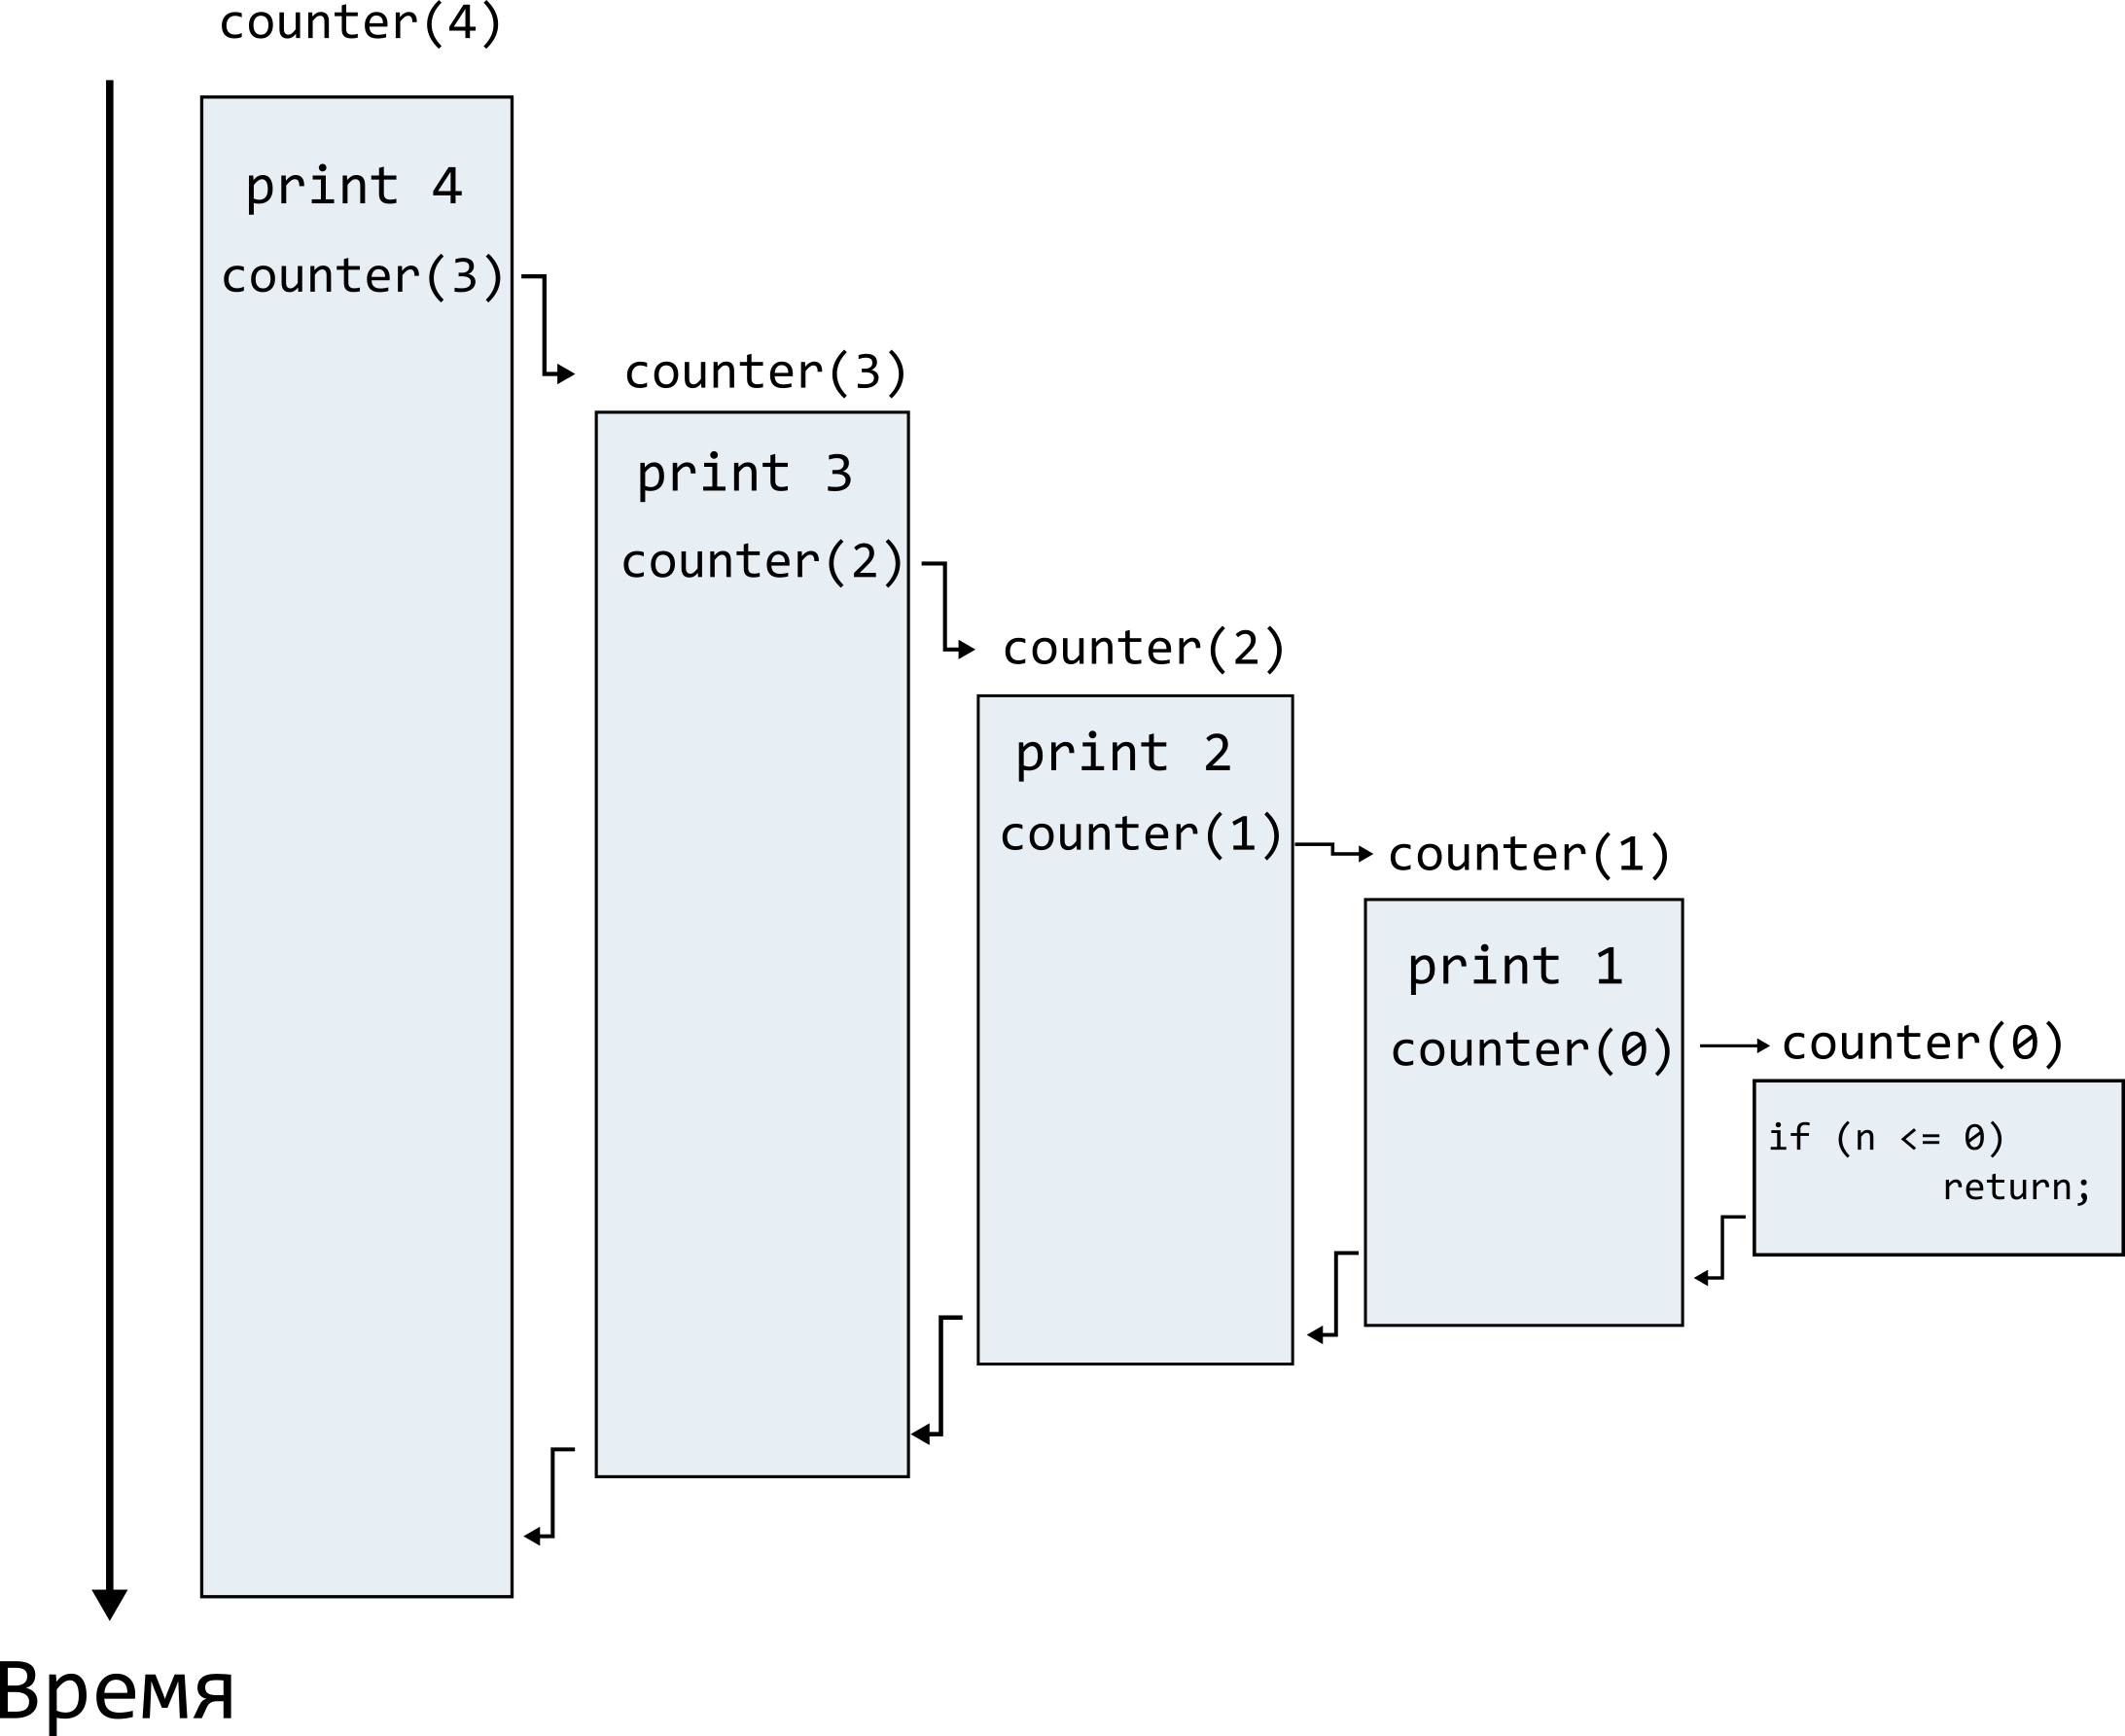
\includegraphics[scale=0.67]{../images/counterini.png}
\end{center}

Схема для функции \texttt{counter}, которая печатает числа по возрастанию выглядит так:
\begin{center}
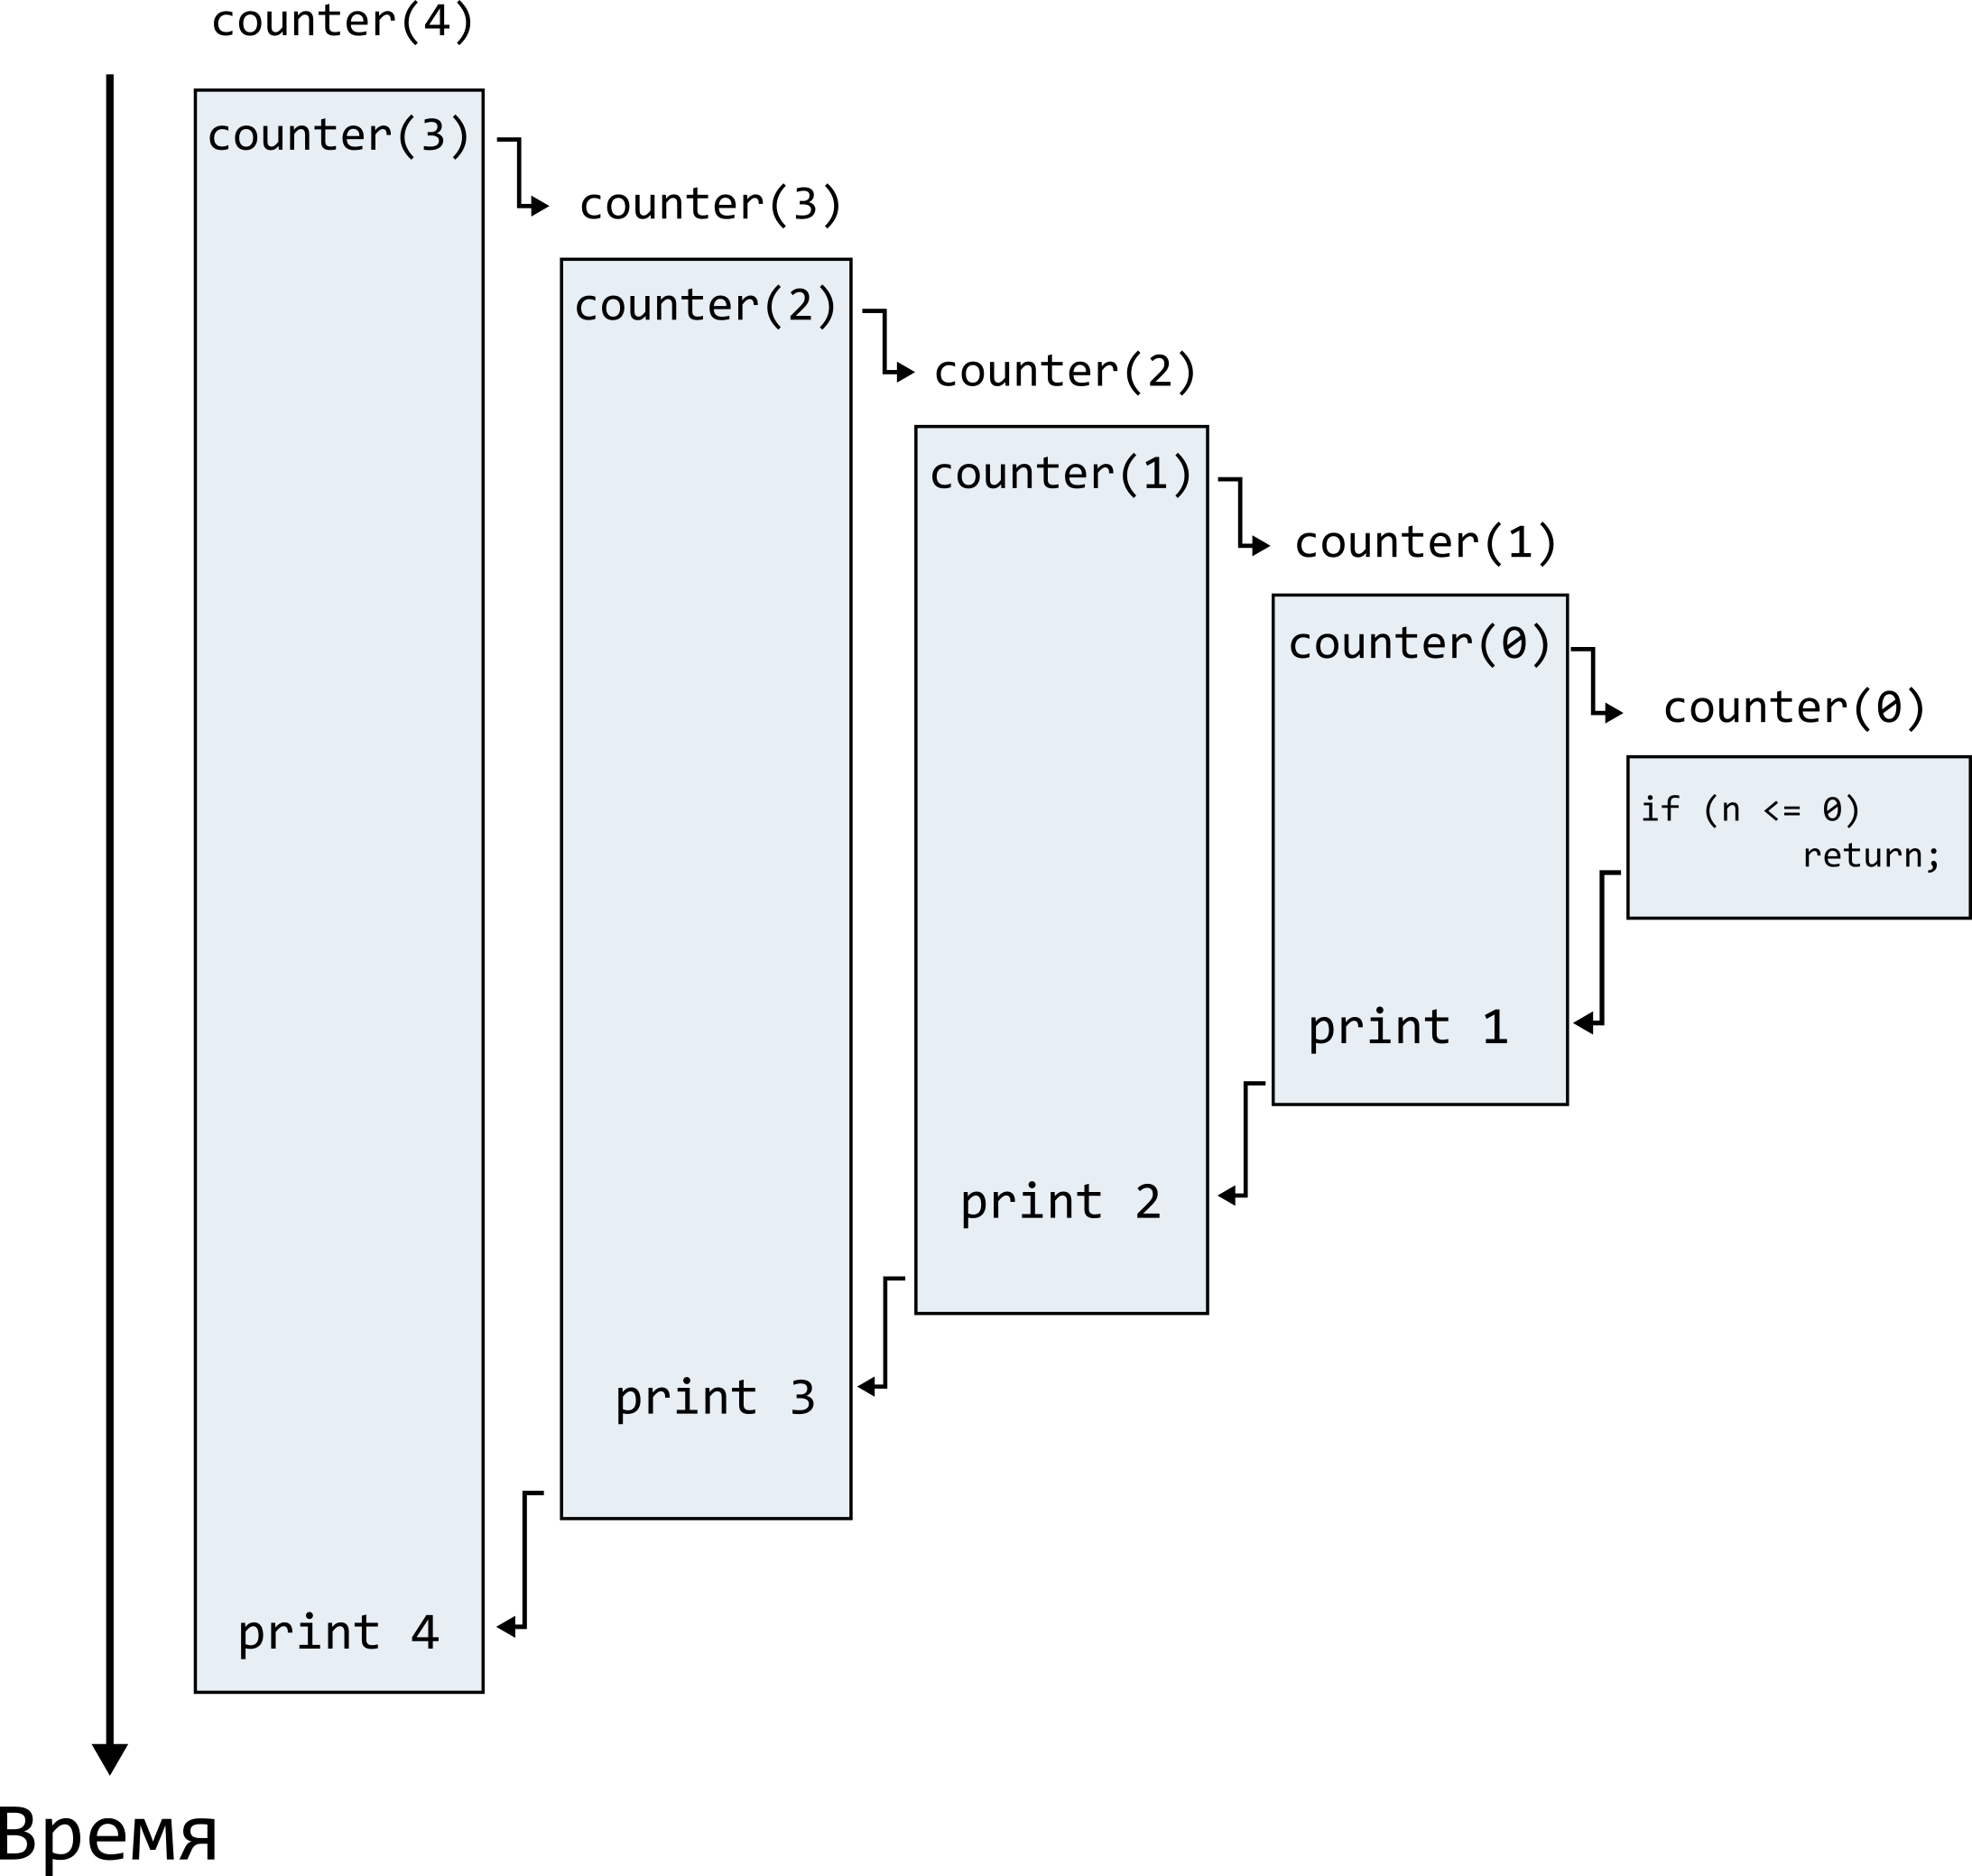
\includegraphics[scale=0.67]{../images/counter.png}
\end{center}

\item \textbf{Факториал:} Напишите функцию \texttt{int fact(int n)}, которая рекурсивно вычисляет факториал числа \texttt{n}. Вызовите эту функцию из main.
\begin{lstlisting}[backgroundcolor = \color{solcolor}]
#include <stdio.h>
int fact(int n) {
    if (n == 0)
        return 1;
    return n * fact(n - 1);
}
int main() {
    printf("%i\n", fact(5));
}
\end{lstlisting}



\item \textbf{Возведение в целую степень:} Напишите функцию \texttt{double power(double a, int n)}, которая рекурсивно возводит число \texttt{a} в целую степень \texttt{n} по формуле:
$$
a^n = a \cdot (a^{n-1})
$$
\begin{lstlisting}[backgroundcolor = \color{solcolor}]
#include <stdio.h>
double power(double a, int n) {
    if (n == 0)
        return 1;
    return a * power(a, n - 1);
}
int main() {
    printf("%lf\n", power(2, 4));
}
\end{lstlisting}


\item \textbf{Скобочки:} Напишите рекурсивную функцию \texttt{brackets}, которая будет печатать некоторую скобочную последовательность. \texttt{brackets(n)} должна сначала печатать \texttt{n} открывающихся скобочек, а затем \texttt{n} закрывающихся. Например, вызов \texttt{bracket(4)} должен напечатать \texttt{(((())))}. \\
Чтобы это сделать рекурсивно нужно сделать следующее:
\begin{itemize}
\item Напечатать открывающуюся скобку
\item Напечатать \texttt{n-1} открывающихся и \texttt{n-1} закрывающихся скобок вызовом рекурсивной функции
\item Напечатать закрывающуюся скобку
\end{itemize}
\begin{lstlisting}[backgroundcolor = \color{solcolor}]
#include <stdio.h>
void brackets(int n) {
    if (n == 0)
        return;
    printf("(");
    brackets(n - 1);
    printf(")");
}
int main() {
    brackets(5);
}
\end{lstlisting}
\newpage
Схема вызовов для этой функции(вызываем \texttt{brackets(3)}):
\begin{center}
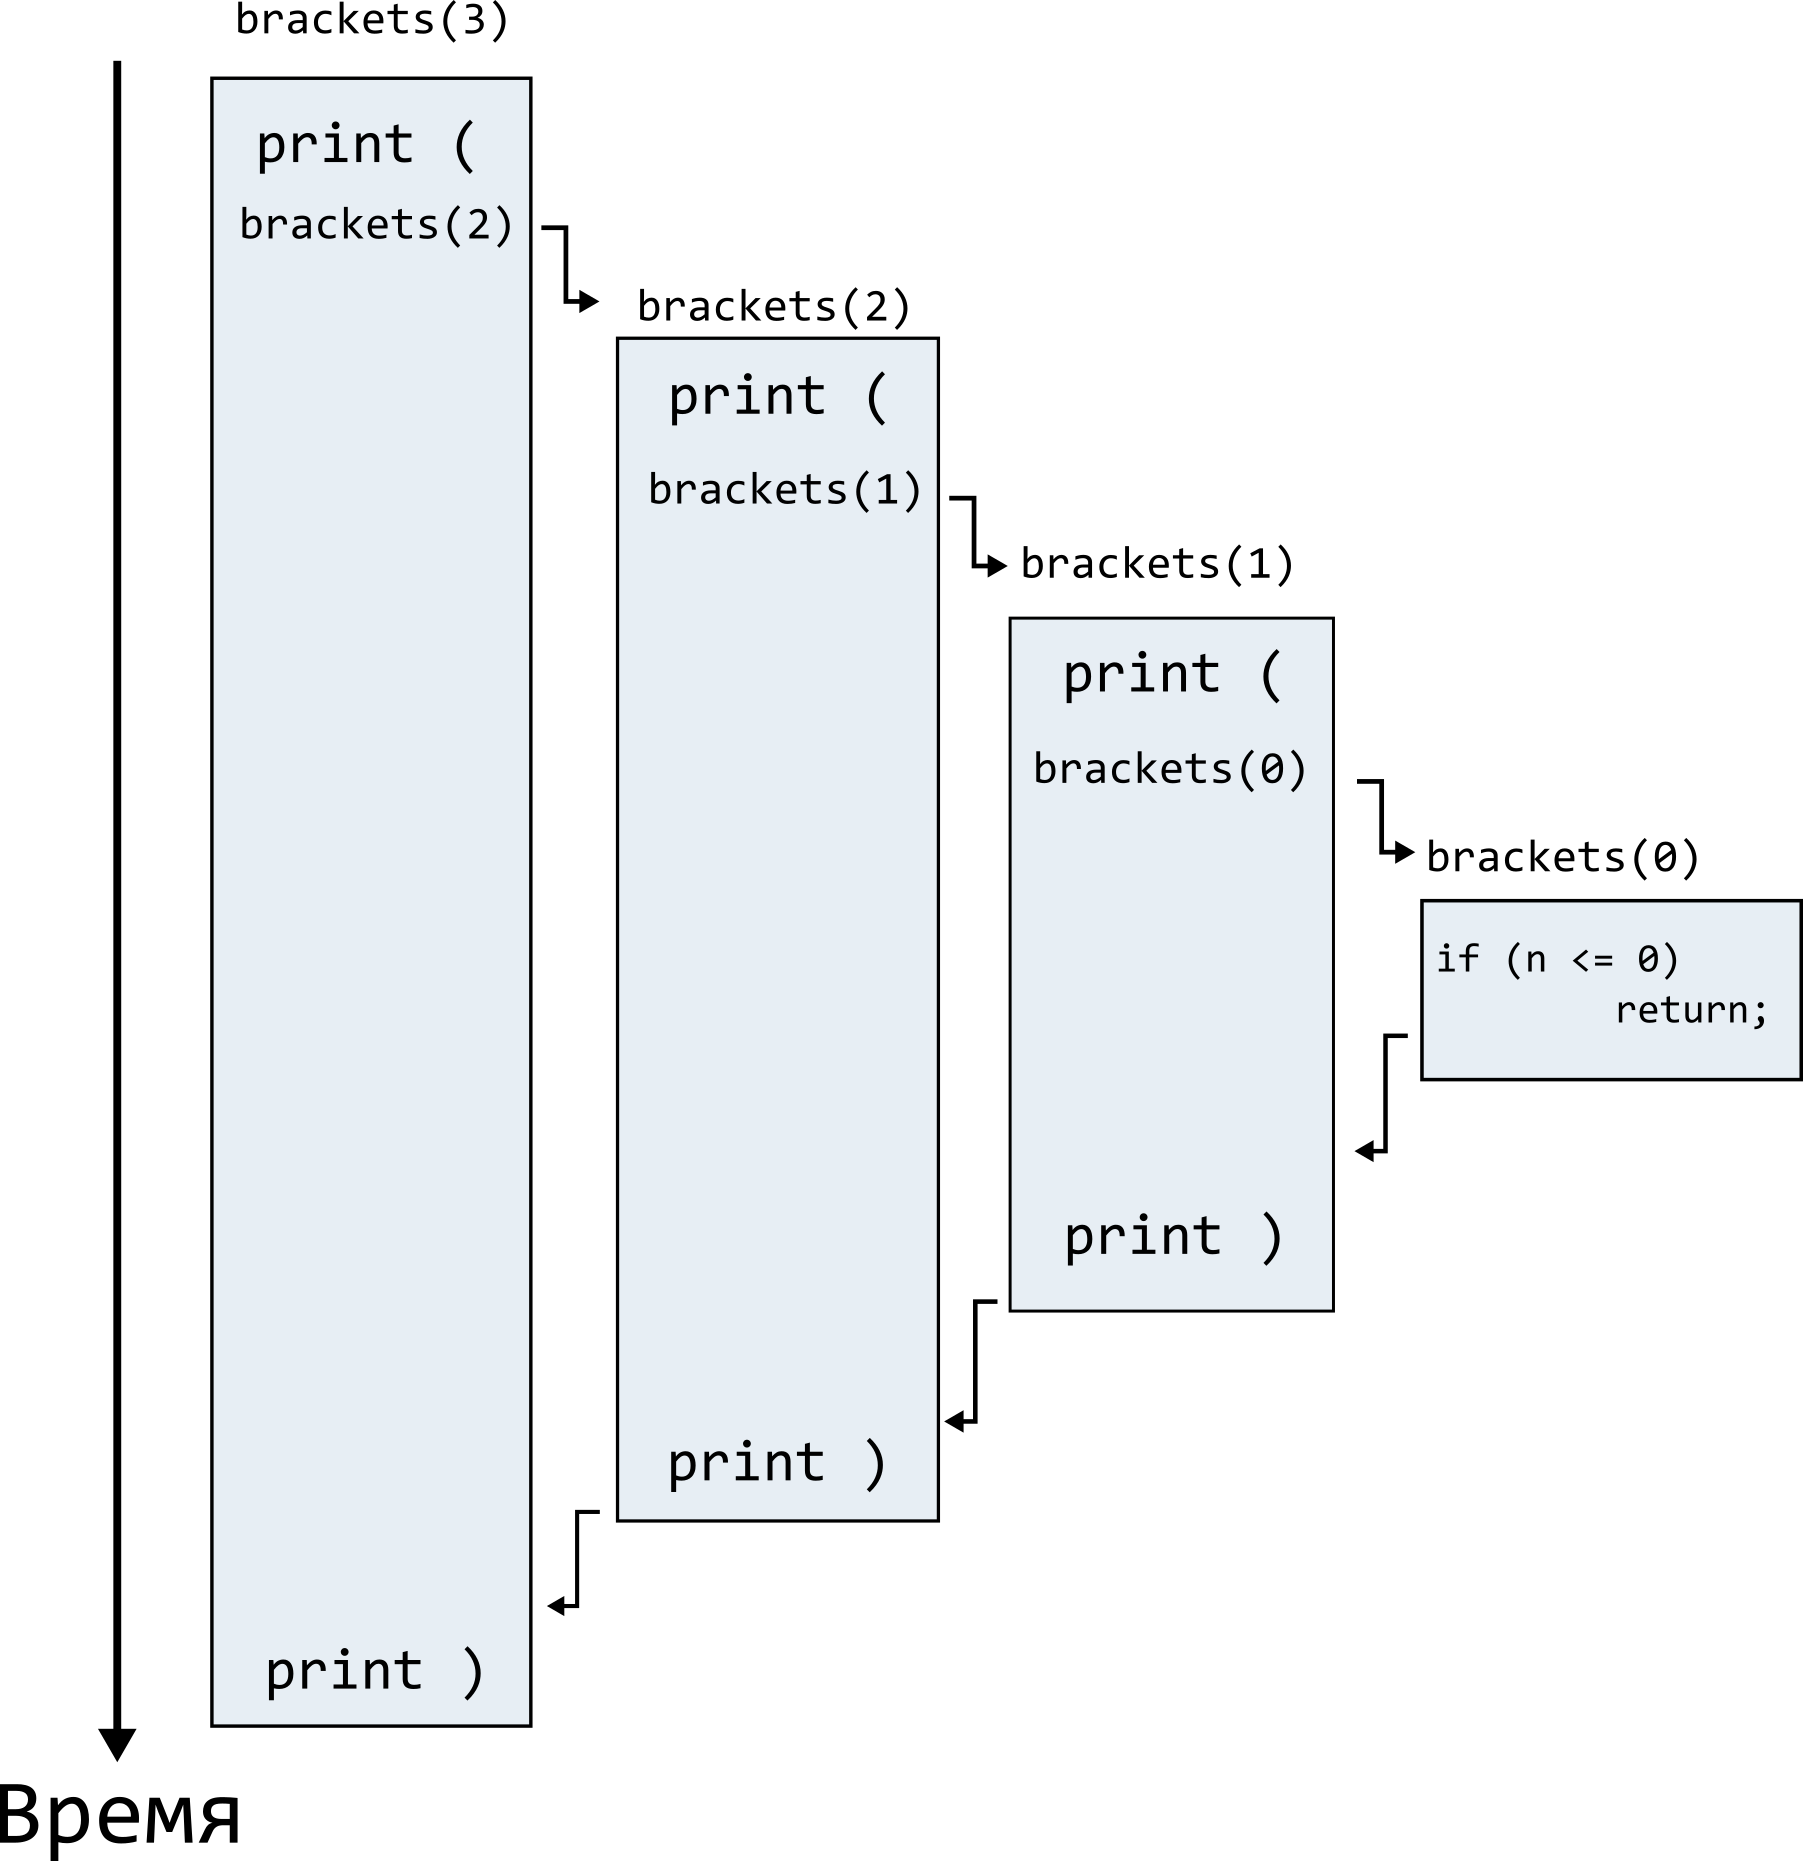
\includegraphics[scale=0.72]{../images/brackets.png}
\end{center}

\item \textbf{Фибоначчи:}
Для вычисления числа Фибоначчи было написано 2 функции. Функция \texttt{fib} вычисляет число Фибоначчи итеративно(то есть с помощью цикла), а функция \texttt{fibrec} вычисляет то же самое рекурсивно. Так как число фибоначчи может быть большим, то в качестве типа данных используется \texttt{long long} вместо \texttt{int}. Переменных типа \texttt{long long} могут хранить числа до примерно $10^{19}$. Числа Фибоначчи до 93-го номера могут храниться в таких переменных.
\begin{lstlisting}
#include <stdio.h>

long long fib(int n) {
    long long a = 0, b = 1;
    for (int i = 1; i < n; ++i) {
        long long temp = a + b;
        a = b;
        b = temp;
    }
    return b;
}
long long fibrec(int n) {
    if (n < 2) {
        return n;
    }
    return fibrec(n - 1) + fibrec(n - 2);
}
int main() {
    printf("%lli\n", fib(20));
    printf("%lli\n", fibrec(20));
}
\end{lstlisting}
Кажется, что обе функции работают, но если посчитать числа Фибоначчи не от 20, а от 60-ти, то рекурсивная функция перестаёт работать. Почему это происходит? \\

Рекурсивная функция вычисления чисел Фибоначчи работает так медленно потому что она по многу раз вычисляет одни и те же значения. На изображении ниже предсталена схема вызовов этой функции для вычисления 10-го числа Фибоначчи.
\begin{center}
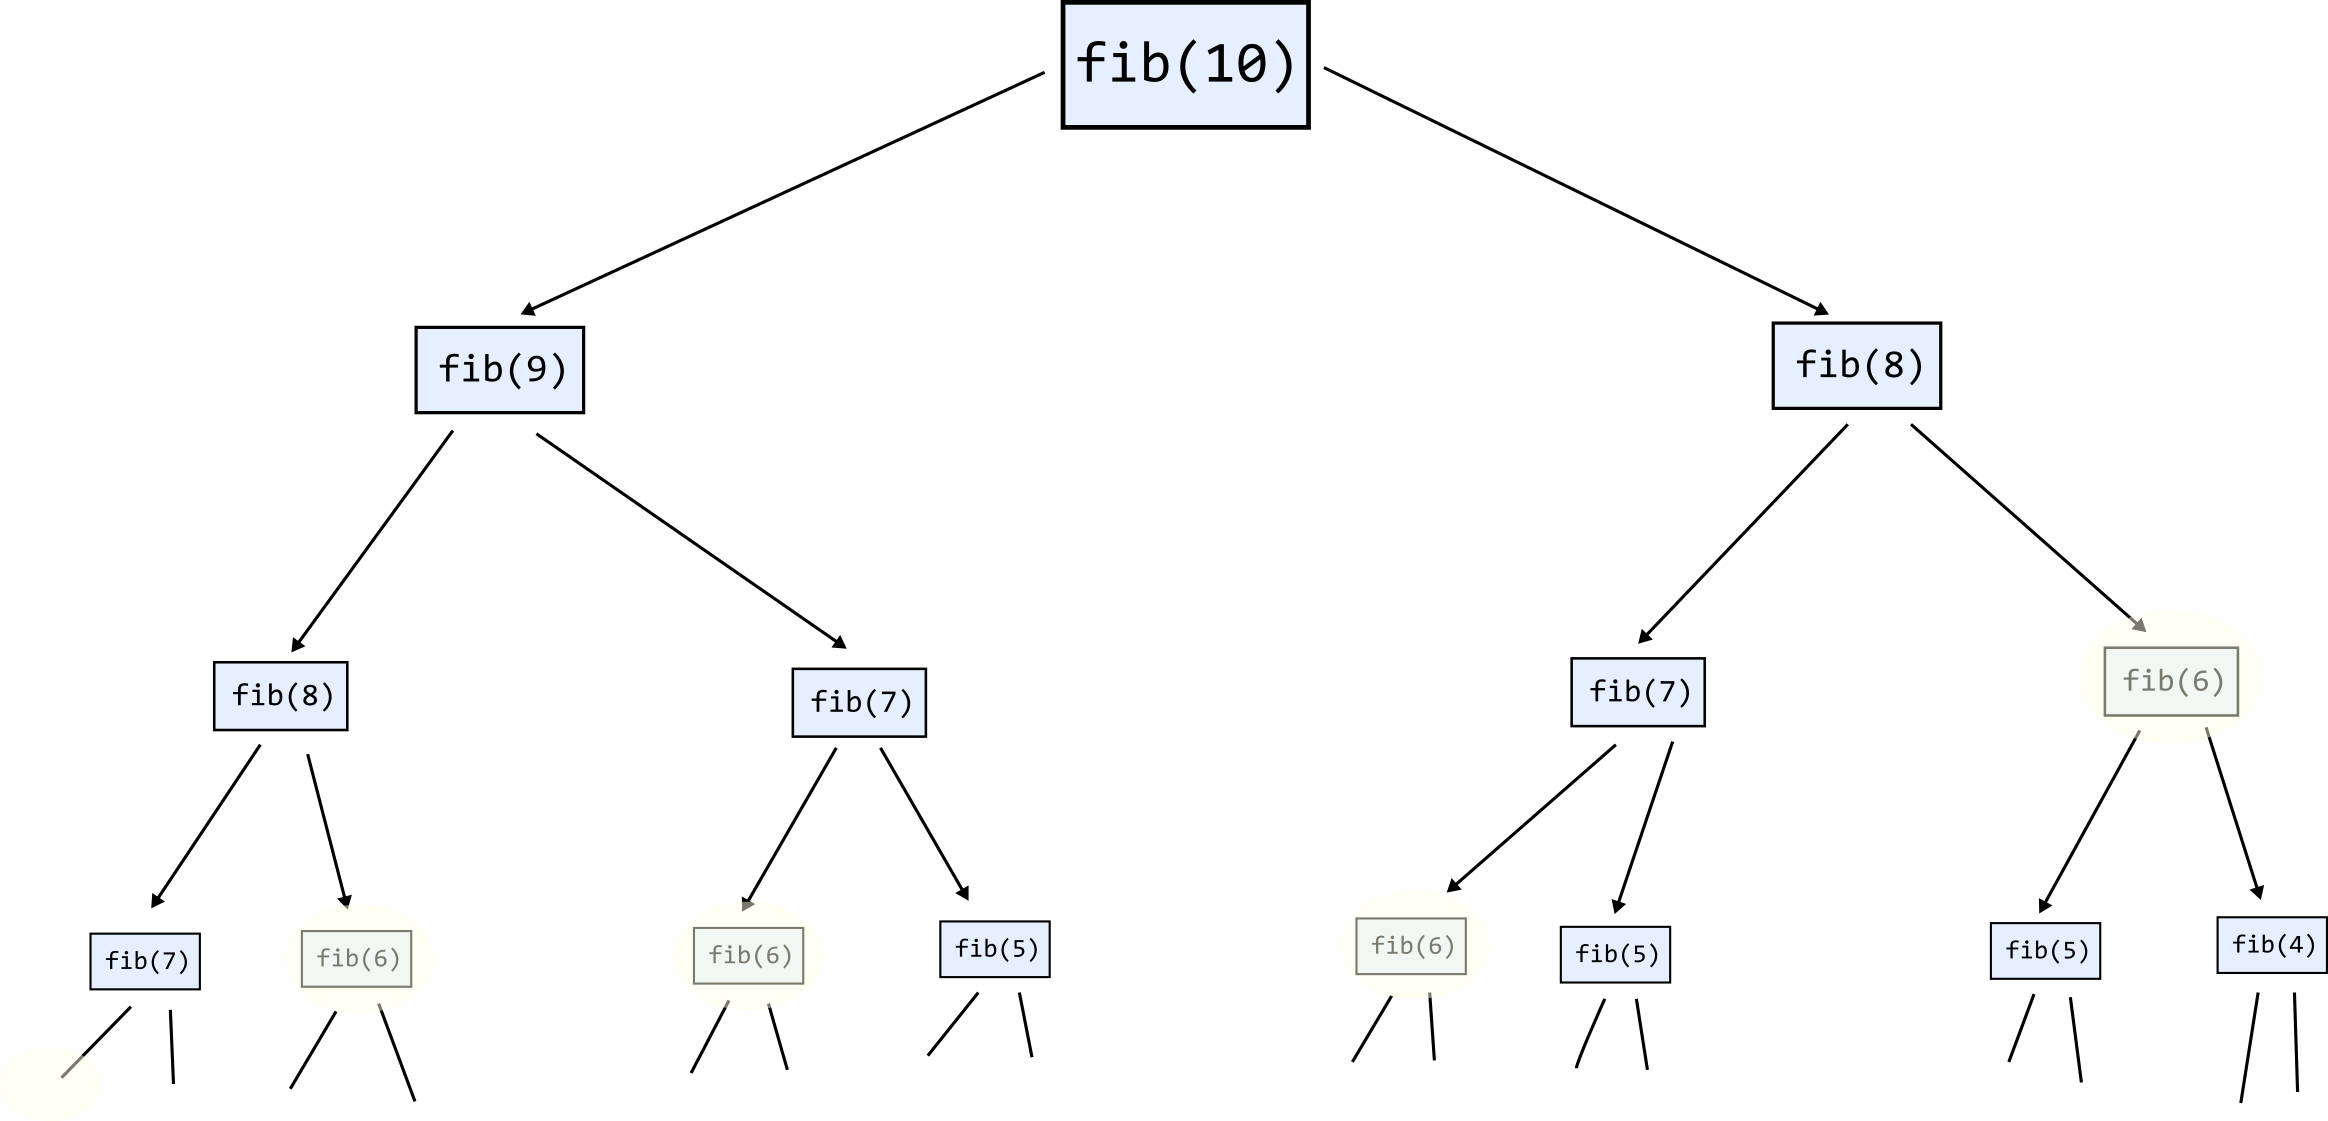
\includegraphics[scale=0.8]{../images/fib.png}
\end{center}
Видно что промежуточные числа Фибоначчи вычисляются заново по много раз. Например, \texttt{fib(6)} вызывается 5 раз в процесе вычисления \texttt{fib(10)}, \texttt{fib(5)} вызывается 8 раз, а меньшие числа Фибоначчи вычисляются ещё чаще. Получается, что количество операций для вычисления одного числа Фибоначчи рекурсивным способом экспоненциально большое.\\

Рекурсивную функцию можно исправить если в процессе выполнения запоминать все промежуточные вычисления и не делать их заново. Для этого заведём глобальный массив \texttt{data} в котором будем хранить все промежуточные числа Фибоначчи. В начале все элементы этого массива равны нулю. Теперь мы продолжаем рекурсию только если мы не вычисляли данное число ранее и \texttt{data[n] == 0}.

\begin{lstlisting}[backgroundcolor = \color{solcolor}]
#include <stdio.h>
long long data[1000];

long long fibrec(int n) {
    if (n < 2) {
        return n;
    }
    if (data[n] == 0) {
        data[n] = fibrec(n - 1) + fibrec(n - 2);
    }
    return data[n];
}

int main() {
    for (int i = 0; i < 1000; ++i)
        data[i] = 0;
    printf("%lli\n", fibrec(90));
}
\end{lstlisting}

\item \textbf{Бинарное возведение в целую степень:} Напишите функцию \texttt{double binpow(double a, int n)}, которая рекурсивно возводит число \texttt{a} в целую степень \texttt{n} по формуле:
\begin{equation*}
a^n = 
\left\{
\begin{alignedat}{2}
 &a \cdot a^{n-1}, &\quad\quad\quad \textup{если } n - \textup{нечётное}\\
 &a^{n/2} \cdot a^{n/2},   & \textup{если } n - \textup{чётное}
\end{alignedat}
\right.
\end{equation*}

Протестируйте функции \texttt{power} и \texttt{binpow} на следующих тестах:
\begin{center}
\begin{tabular}{ l | l }
 вход & выход \\ \hline
 \texttt{2 4} & \texttt{16}  \\ 
 \texttt{1.05 100} & \texttt{131.501}  \\ 
 \texttt{1.00001 1000000} & \texttt{22025.364}  \\
 \texttt{1.00000001 2000000000} & \texttt{485165075.539}  \\
\end{tabular}
\end{center}
Какая из этих функций более эффективна?

\begin{lstlisting}[backgroundcolor = \color{solcolor}]
#include <stdio.h>

double binpow(double a, int n) {
    if (n == 0) {
        return 1;
    }
    if (n % 2) {
        return a * binpow(a, n - 1);
    }
    else {
        double temp = binpow(a, n / 2);
        return temp * temp;
    }
}

int main() {
    printf("%lf\n", binpow(1.05, 100));
}
\end{lstlisting}
В этой функции важно не сделать ту же ошибку, что встретилась в задаче вычисления чисел Фибоначчи, и не вызвать \texttt{binpow(a, n/2)} два раза.\\

Для вычисления \texttt{n}-й степени функции \texttt{power} требуется порядка $n$ операции умножения, а функции \texttt{binpow} для того же самого требуется порядка $\log_2(n)$ операций. Конечно, функция \texttt{binpow} намного быстрее.
\end{itemize}




\newpage
\section*{Часть 3: Передача массива в функцию}
Массивы можно передавать в функции. Однако, передача массива в функцию в языке \texttt{C} устроена таким образом, что узнать размер массива внутри функции нельзя. Поэтому размер массива нужно тоже передавать в функцию вместе с массивом.\\

Пример двух функций: одна печатает массив на экран, другая прибавляет ко всем элементам массива \texttt{1}.
\begin{lstlisting}
#include <stdio.h>
void print_array(int array[], int size) {
    for (int i = 0; i < size; ++i) {
        printf("%i ", array[i]);
    }
    printf("\n");
}
void inc(int array[], int size) {
    for (int i = 0; i < size; ++i) {
        array[i] += 1;
    }
}
int main() {
    int a[10] = {4, 8, 15, 16, 23, 42};
    print_array(a, 6);
    inc(a, 6);
    print_array(a, 6);
}
\end{lstlisting}


\subsubsection*{Задачи:}
Все эти функции нужно писать в одном файле. Также всех их нужно протестировать, вызвав из функции \texttt{main}. Все эти функции не должны ничего печатать, а должны просто изменять массив или возвращать значения. Вся печать должно совершаться посредством вызова функции \texttt{print\_array} из функции \texttt{main}.
\begin{itemize}
\item Напишите функцию \texttt{mult2}, которая принимает на вход массив и его размер, а затем умножает каждый элемент массива на \texttt{2}. Протестируйте эту функцию в функции \texttt{main}. Используйте \texttt{print\_array} для печати массива.
\item Напишите функцию \texttt{sqr}, которая принимает на вход массив и его размер, а затем возводит каждый элемент массива в квадрат.
\item Напишите функцию \texttt{add\_x}, которая принимает на вход массив, его размер и некоторое число \texttt{x}, а затем прибавляет ко всем элементам массива это число.
\item Напишите функцию \texttt{sum}, которая принимает на вход массив и его размер и возвращает сумму элементов этого массива.
\item Напишите функцию \texttt{max}, которая возвращает максимальный элемент массива.
\item Напишите функцию \texttt{int sum\_subarray(int array[], int l, int r)}, которая принимает на вход массив и границы подмассива и возвращает сумму элементов данного подмассива. Например, сумма подмассива \texttt{a[1, 4]} равна \texttt{39}.

\item Напишите функцию \texttt{void add\_array(int C[], int A[], int B[], int size)}. Эта функция должна складывать массивы \texttt{A} и \texttt{B} и записывать результат в массив \texttt{C}. 
\end{itemize}
\newpage
\begin{lstlisting}[backgroundcolor = \color{solcolor}]
#include <stdio.h>
void print_array(int array[], int size) {
    for (int i = 0; i < size; ++i) {
        printf("%i ", array[i]);
    }
    printf("\n");
}
void inc(int array[], int size) {
    for (int i = 0; i < size; ++i) {
        array[i] += 1;
    }
}
void mult2(int array[], int size) {
    for (int i = 0; i < size; ++i) {
        array[i] *= 2;
    }
}
void sqr(int array[], int size) {
    for (int i = 0; i < size; ++i) {
        array[i] *= array[i];
    }
}
void add_x(int array[], int size, int x) {
    for (int i = 0; i < size; ++i) {
        array[i] += x;
    }
}
int sum_array(int array[], int size) {
    int result = 0;
    for (int i = 0; i < size; ++i) {
        result += array[i];
    }
    return result;
}
int sum_subarray(int array[], int l, int r) {
    int result = 0;
    for (int i = l; i < r; ++i) {
        result += array[i];
    }
    return result;
}

int max(int a, int b) {
    return a > b ? a : b;
}
int max_array(int array[], int size) {
    int result = array[0];
    for (int i = 0; i < size; ++i)
        result = max(result, array[i]);
    return result;
}

void add_array(int C[], int A[], int B[], int size) {
    for (int i = 0; i < size; ++i) {
        C[i] = A[i] + B[i];
    }
}


int main() {
    int a[10] = {4, 8, 15, 16, 23, 42};
    print_array(a, 6);
    printf("Sum       %i\n", sum_array(a, 6));
    printf("Sum[1,4]  %i\n", sum_subarray(a, 1, 4));
    printf("Max       %i\n", max_array(a, 6));

    printf("Square:\n");
    sqr(a, 6);
    print_array(a, 6);
    
    
    printf("\nAdd arrays:\n");
    int A[6] = {4, 8, 15, 16, 23, 42};
    int B[6] = {5, 9,  1, 55, 90, 20};
    int C[6];
    add_array(C, A, B, 6);
    print_array(C, 6);
}
\end{lstlisting}


\section*{Часть 4: Рекурсия на подотрезках}
Рекурсию можно применять и на массивах. В примере ниже написана функция \texttt{sumrec}, которая рекурсивно вычисляет сумму подмассива. Для этого она делает следующее:
\begin{itemize}
\item[--] Если в подмассиве 1 элемент, то нужно просто вернуть этот элемент.
\item[--] Вычисляет середину подмассива
\item[--] Рекурсивно вызывает себя для вычисления сумм левой половины подмассива и правой половины.
\item[--] Возвращает сумму левой и правой половины 
\end{itemize}
\begin{lstlisting}
#include <stdio.h>

int sumrec(int array[], int l, int r) {
    if (r - l == 1) {
        return array[l];
    }
    int mid = l + (r - l) / 2;
    return sumrec(array, l, mid) + sumrec(array, mid, r); 
}

int main() {
    int a[6] = {4, 8, 15, 16, 23, 42};
    printf("%i\n", sumrec(a, 0, 6));
}
\end{lstlisting}
Все задачи можно решить как с помощью цикла, так и с помощью рекурсии. Чаще решение с помощью цикла является более понятным и простым, но бывают задачи, решение которых проще сделать с помощью рекурсии.
\subsubsection*{Задачи:}
\begin{itemize}
\item Напишите рекурсивную функцию, которая вычисляет максимум на подмассиве.
\begin{lstlisting}[backgroundcolor = \color{solcolor}]
#include <stdio.h>
int max(int a, int b) {
    return a > b ? a : b;
}

int maxrec(int array[], int l, int r) {
    if (r - l == 1) {
        return array[l];
    }
    int mid = l + (r - l) / 2;
    return max(maxrec(array, l, mid), maxrec(array, mid, r)); 
}

int main() {
    int a[6] = {4, 8, 95, 16, 23, 42};
    printf("%i\n", maxrec(a, 0, 6));
}
\end{lstlisting}
\item Функция сортировки выбором выглядит так (нужно добавить функцию \texttt{print\_array}):
\begin{lstlisting}
#include <stdio.h>
void selection_sort(int array[], int size) {
    for (int i = 0; i < size; ++i) {
        int min_index = i;
        for (int j = i + 1; j < size; ++j)
            if (array[j] < array[min_index])
                min_index = j;
        
        int temp = array[i];
        array[i] = array[min_index];
        array[min_index] = temp;
    }
}
int main() {
    int a[10] = {15, 11, 54, 8, 1, 6, 5, 97, 1, 22};
    print_array(a, 10);
    selection_sort(a, 10);
    print_array(a, 10);
}
\end{lstlisting}
Напишите функцию \texttt{selection\_sort\_rec}, которая будет сортировать выбором, но рекурсивно.

\newpage
\begin{lstlisting}[backgroundcolor = \color{solcolor}]
#include <stdio.h>
void print_array(int array[], int size) {
    for (int i = 0; i < size; ++i) {
        printf("%i ", array[i]);
    }
    printf("\n");
}
void selection_sort_rec(int array[], int l, int r) {
    if (r - l <= 1) {
        return;
    }
    int min_index = l;
    for (int j = l + 1; j < r; ++j)
        if (array[j] < array[min_index])
            min_index = j;
    
    int temp = array[l];
    array[l] = array[min_index];
    array[min_index] = temp;
    
    selection_sort_rec(array, l + 1, r);
}
int main() {
    int a[10] = {15, 11, 54, 8, 1, 6, 5, 97, 1, 22};
    print_array(a, 10);
    selection_sort_rec(a, 0, 10);
    print_array(a, 10);
}
\end{lstlisting}
\end{itemize}
\newpage
\section*{Часть 5: Передача по указателю}
Отличие массивов от других переменных заключается в том, что при их изменении внутри функции, они меняются и вне функций. С обычными переменными это не работает. Для того чтобы можно было менять переменные внутри функций нужно использовать указатели.
Пример программы, которая создаёт указатель \texttt{p}. Этот указатель хранит адрес переменной \texttt{a}.
\begin{lstlisting}
#include <stdio.h>
int main() {
    int a = 100;
    int* p = &a;
	
    *p = 321;
    printf("%d\n", a);     
}
\end{lstlisting}
\texttt{int*} -- это тип переменной \texttt{p} -- указатель на \texttt{int}. \\
\texttt{*p} -- в этой строки символ \texttt{*} имеет другой смысл. Она означает, что нужно пойти по адресу, который хранится в \texttt{p} и воспринимать эту область памяти как число \texttt{int}.

\begin{itemize}
\item Создайте переменную \texttt{b} типа \texttt{float} и присвойте ей какое-либо значение. Создайте переменную \texttt{p} типа указатель на \texttt{float} (\texttt{p} - это сокращение от pointer - указатель)  и присвойте ей значение -- адрес переменной \texttt{b}. Измените переменную \texttt{b}, используя только переменную \texttt{p}.
\begin{lstlisting}[backgroundcolor = \color{solcolor}]
#include <stdio.h>
int main() {
    float b = 123.45;
    float* p = &b;
    *p /= 2;
    printf("%f\n", b);
}
\end{lstlisting}
\item Создайте переменную \texttt{pp} и присвойте ей значение -- адрес переменной \texttt{p}. Измените переменную \texttt{b}, используя только переменную \texttt{pp}.
\begin{lstlisting}[backgroundcolor = \color{solcolor}]
#include <stdio.h>
int main() {
    float b = 123.45;
    float* p = &b;
    float** pp = &p;
    **pp /= 2;
    printf("%f\n", b);
}
\end{lstlisting}
\end{itemize}

\newpage
Пример передачи в функцию с помощью указателей. Пытаемся увеличить переменную на 10.
\begin{lstlisting}
#include <stdio.h>
void add10_wrong(int a){
    a += 10;
}
void add10_right(int* p){
    *p += 10;
}
int main() {
    int a = 80;
    add10_wrong(a);
    printf("%d\n", a); 
	    
    add10_right(&a);
    printf("%d\n", a); 
}
\end{lstlisting}

\begin{itemize}
\item Написать функцию \texttt{void mult2(int* p)}, которая удваивает число, поступающее на вход, используя указатель на эту переменную. Протестируйте эту функцию в функции \texttt{main}.

\begin{lstlisting}[backgroundcolor = \color{solcolor}]
#include <stdio.h>
void mult2(int* p) {
    *p *= 2;
}
int main() {
    int a = 10;
    mult2(&a);
    printf("%i\n", a);
}
\end{lstlisting}
\item Написать функцию \texttt{swap}, которая меняет значения 2-х переменных типа \texttt{int} местами. Используйте эту функцию в функции \texttt{main}.
\begin{lstlisting}[backgroundcolor = \color{solcolor}]
#include <stdio.h>
void swap(int* pa, int* pb) {
    int temp = *pa;
    *pa = *pb;
    *pb = temp;
}
int main() {
    int a = 10, b = 20;
    printf("%i %i\n", a, b);
    swap(&a, &b);
    printf("%i %i\n", a, b);
}
\end{lstlisting}
\end{itemize}

\end{document}
